%%% Для сборки выполнить 2 раза команду: pdflatex <имя файла>

\documentclass[a4paper,12pt]{article}

\usepackage[margin=1in]{geometry}
\usepackage{ucs}
\usepackage[utf8x]{inputenc}
\usepackage[english, russian]{babel}
%\usepackage{cmlgc}
\usepackage{graphicx}
\usepackage{listings}
\usepackage{xcolor}
\usepackage{wrapfig}
\usepackage{sidecap}
%\usepackage{courier}

\makeatletter
\renewcommand\@biblabel[1]{#1.}
\makeatother

\newcommand{\myrule}[1]{\rule{#1}{0.4pt}}
\newcommand{\sign}[2][~]{{\small\myrule{#2}\\[-0.7em]\makebox[#2]{\it #1}}}

% Поля
\usepackage[top=20mm, left=30mm, right=10mm, bottom=20mm, nohead]{geometry}
\usepackage{indentfirst}

% Межстрочный интервал
\renewcommand{\baselinestretch}{1.50}

% Согласно ГОСТу в заголовках таблиц, листинго кода, рисунков
% в качестве разделителя номера и текста заголовка используется тире 
\usepackage[labelsep=endash]{caption} 
\captionsetup[table]{skip=1ex}

% Размер полосы разделителя между столбцами таблицы по умолчанию
\setlength{\tabcolsep}{1em}

% Формат листинга по умолчанию
\lstdefinestyle{mylisting}{%
    basicstyle=\ttfamily,
    columns=fullflexible,
    keepspaces=true,
    commentstyle=\normalshape,
    keywordstyle=\bfseries,
    showstringspaces=false,
    captionpos=t,
    belowcaptionskip=1.5ex,
    frame=lines
}

\begin{document}

%%%%%%%%%%%%%%%%%%%%%%%%%%%%%%%
%%%                         %%%
%%% Начало титульного листа %%%

\thispagestyle{empty}
\begin{center}


\renewcommand{\baselinestretch}{1}
{\large
{\sc Петрозаводский государственный университет\\
Институт математики и информационных технологий\\
	Кафедра Информатики и математического обеспечения
}
}

\end{center}


\begin{center} 
Направление подготовки бакалавриата \\
09.03.04 Программная инженерия \\
Профиль направления подготовки бакалавриата \\
``Системное и прикладное программное обеспечение''

\end{center}

\vfill

\begin{center}
{\normalsize Курсовая работа по теме:} \\
\medskip

%%% Название работы %%%
	{\Large \sc {Создание бота на платформе Discord}} \\
\end{center}

\medskip

\begin{flushright}
\parbox{11cm}{%
\renewcommand{\baselinestretch}{1.2}
\normalsize
	Выполнил\\
%%% ФИО студента %%%
студент группы 22207:
\begin{flushright}
	А. П. Бровкин \sign[подпись]{4cm}
\end{flushright}
%%%%%%%%%%%%%%%%%%%%%%%%%
% девушкам применять "Выполнила" и "студентка"
%%%%%%%%%%%%%%%%%%%%%%%%%






Научный руководитель\\ к.т.н., доцент кафедры ИМО:\\
%%% степень, звание ФИО научного руководителя %%%
%%% Первый руководитель 
%%% {автор задачи, если выбран мини проект} 
\begin{flushright}
{ C. А. Марченков \sign[подпись]{4cm} }
\end{flushright}


Итоговая оценка
\begin{flushright}
  \sign[оценка]{4cm}
\end{flushright}
}
\end{flushright}

\vfill

\begin{center}
\large
    Петрозаводск --- 2022
\end{center}

%%% Конец титульного листа  %%%
%%%                         %%%
%%%%%%%%%%%%%%%%%%%%%%%%%%%%%%%

%%%%%%%%%%%%%%%%%%%%%%%%%%%%%%%%
%%%                          %%%
%%% Текст отчета             %%%


\newpage
\tableofcontents

\newpage
\section*{Введение}
\addcontentsline{toc}{section}{Введение}
\large {

Discord - это бесплатное приложение для голосового, видео и текстового общения, которым пользуются десятки миллионов людей, чтобы общаться с друзьями и участниками сообществ.

Несмотря на то, что изначально Discord создавался для игрового сообщества, его аудитория на сегодняшний день намного разнообразнее. Ежедневно люди используют Discord для самых разных целей: от обсуждения художественных проектов и семейных поездок до проверки домашних заданий и организации психологических консультаций. Discord открыт для сообществ самых разных размеров, но наиболее широко используется небольшими активными группами людей для ежедневного общения.

Большинство серверов являются частными, куда можно попасть только по приглашению и где друзья и участники сообществ могут общаться и проводить время вместе. Существуют и более крупные и открытые сообщества, обычно сосредоточенные вокруг определенных тем, например, популярных игр, таких как Minecraft и CS:GO. Здесь люди могут общаться о чем угодно и свободно делиться своим опытом использования Discord.

Люди любят Discord, потому что он является общим домом для их друзей и сообществ, в которых они состоят. Это место, где можно быть самим собой и проводить время с людьми, разделяющими их интересы и увлечения. Здесь нет алгоритма, определяющего, что именно они должны видеть, нет бесконечной прокрутки и новостной ленты. Общение в Discord основано именно на общих интересах.

Также Discord предоставляет обширный API, который разработчики могут использовать для создания весьма функциональных Discord-ботов, а другие пользователи в последствии могут его использовать для улучшения своего сервера (к примеру бот предаставляющий музыку).} \\ \\


\textbf{Цели:}
\begin{itemize}
    \item Приобрести навыки и опыт работы с платформой Discord, с точки зрения разработчика
    \item Повысить свою квалификацию по ходу работы с JavaScript, Node.js, JSON
    \item Закрепить имеющиеся навыки во время работы с:
    \begin{itemize}
     \item Языками разметки: LaTeX, Beamer, HTML
    \item Языком программирования: JavaScript
    \item Языком таблиц стиле: CSS
    \item Веб-сервисом для хостинга: GitHub
    \end{itemize}
\end{itemize}

\textbf{Задачи:} 
\begin{itemize}
    \item Создание дискорд сервера для тестирования работы бота
    \item Создание бота
    \item Активация бота и его тестирование 
    \item Добавление большего функционала (добавляем команды)
    \item Создание сайта для скачивания бота другим пользователям
    \item Проанализировать полученные результаты и сформулировать выводы, что удалось реализовать, что неудалось, какой получили опыт в результате работы
    \item Создание документации
    \item Отправление документации и кода на репозиторий GitHub
\end{itemize}

\newpage
\section{Реализация}

\subsection{Создание дискорд сервера }

Нажимаем на кнопку "+" в левой колонке \\
Следующее появившееся окно предложит две опции: "Создать" или "Войти". В данном случае выбираем "Создать" \\
После выбора между "Создать" и "Войти", указываем название сервера, а также меняем его иконку, указав ее из своих файлов. \\
Также можем указать регион сервера, но для работы это не пригодится
\\
\\
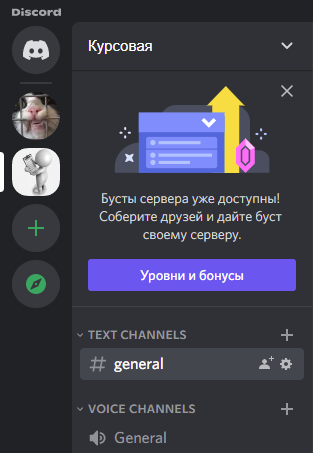
\includegraphics[width = 350px, height=350px]{pictures/Server.png}

\newpage
\subsection{Создание бота}
Чтобы создать бота, перейдём в Discord для разработчиков.Сначала вам нужно создать приложение, затем в этом приложении создать бота и настроить для него разрешения, и только после этого — добавлять бота на сервер. \\
\begin{itemize}
    \item 1. На вкладке Applications выбираем New Application.
    \item 2. Вводим название будущего приложения и нажимаем Create.
    \item 3. Приложение создано. Переходим на вкладку Bot и нажимаем Add Bot, чтобы добавить нового бота.
    \item 4. Соглашаемся добавить бота в наше приложение.
    \item 5. Бот создан. На вкладке Bot отобразится вся информация о нем. Тут можно изменить его имя, добавить изображение и скопировать токен бота. Этот токен понадобится нам для настройки модуля Discord.
    Сохраняем токен бота
    \item 6. Теперь перейдём на вкладку OAuth2 — тут можно настроить разрешения и получить ссылку на нашего бота. В разделе SCOPES выберим bot, в BOT PERMISSIONS отметим разрешения, которые предоставим ему. После  копируем автоматически сгенерированную Discord ссылку.
    \item 7. Перейдём по ссылке и добавим бота на сервер
    \item 8. На сервере бот оставил приветственное сообщение — значит, что он успешно добавлен и функционирует.
\end{itemize}
\noindent


\centerline{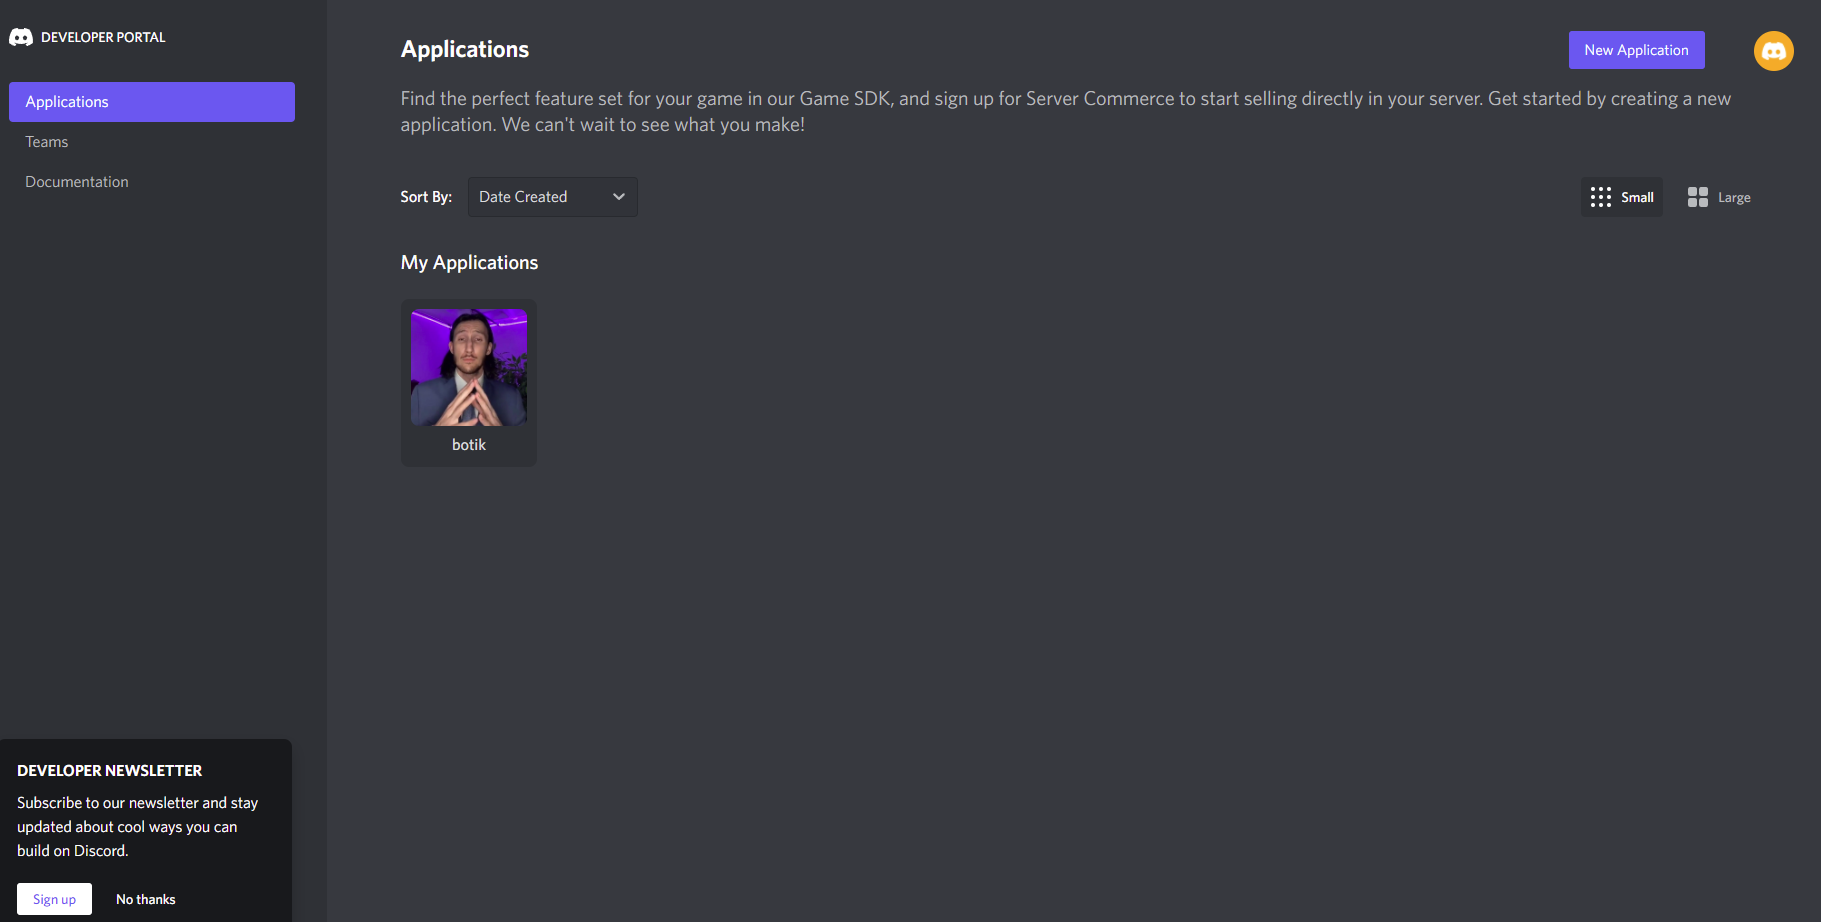
\includegraphics[width = 450px]{pictures/application.png}} \\
\vspace{5mm}
\centerline{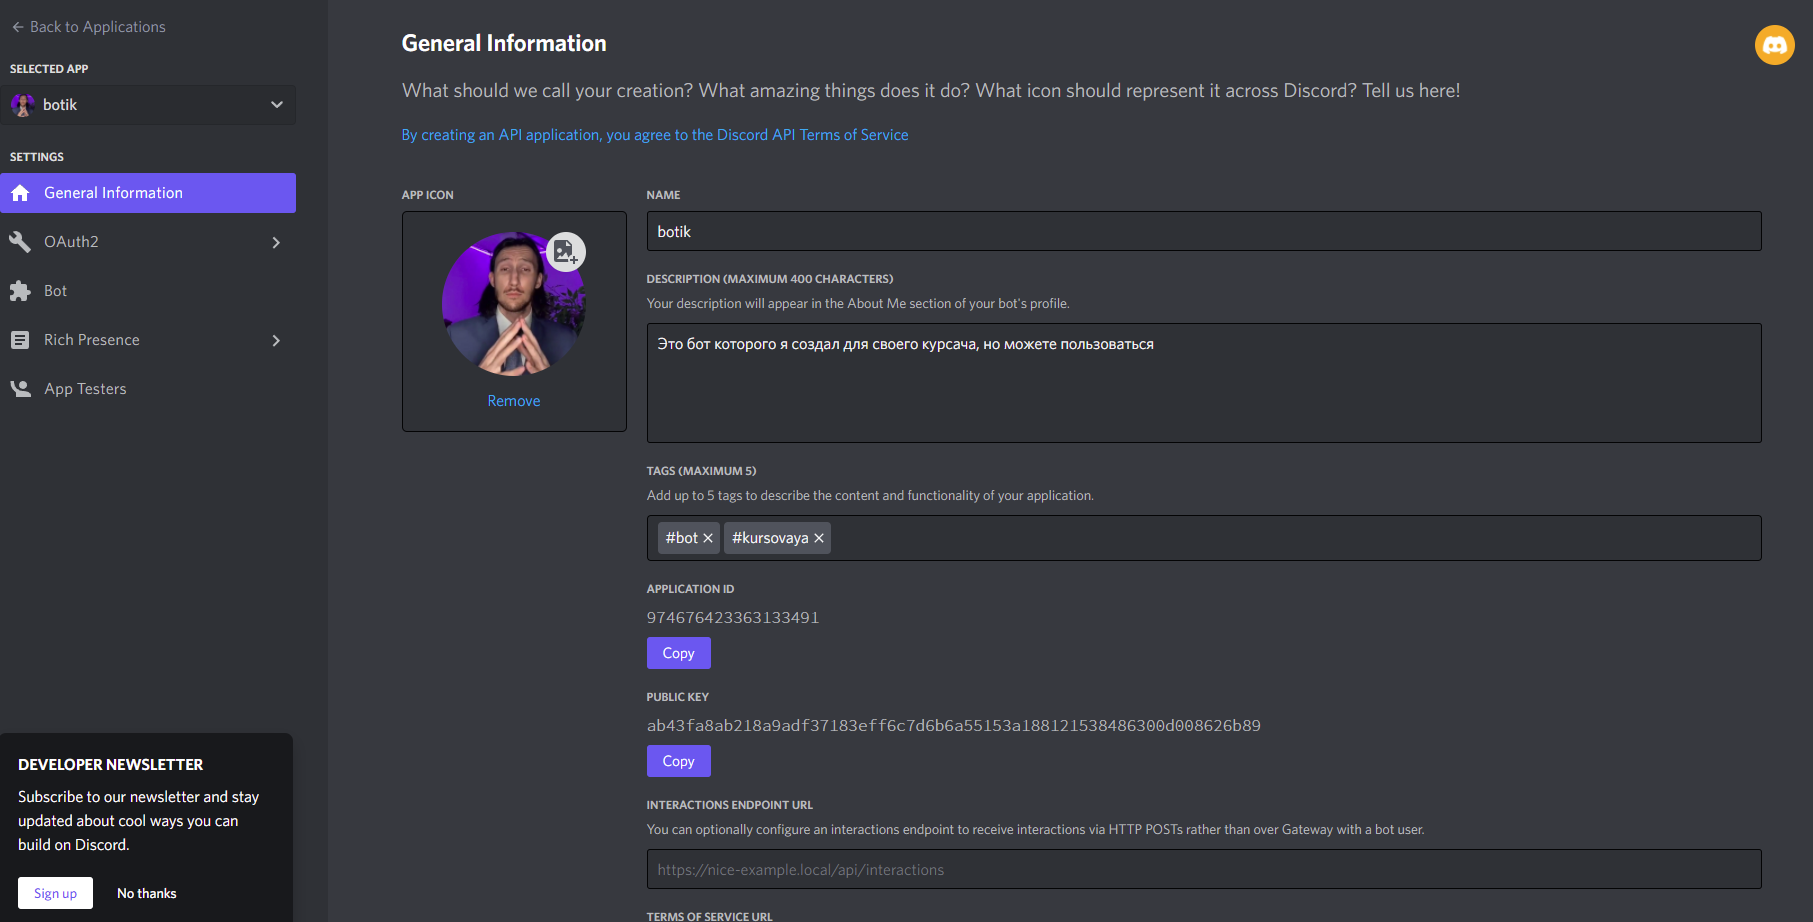
\includegraphics[width = 450px]{pictures/bot.png}} \\
\vspace{5mm}
\centerline{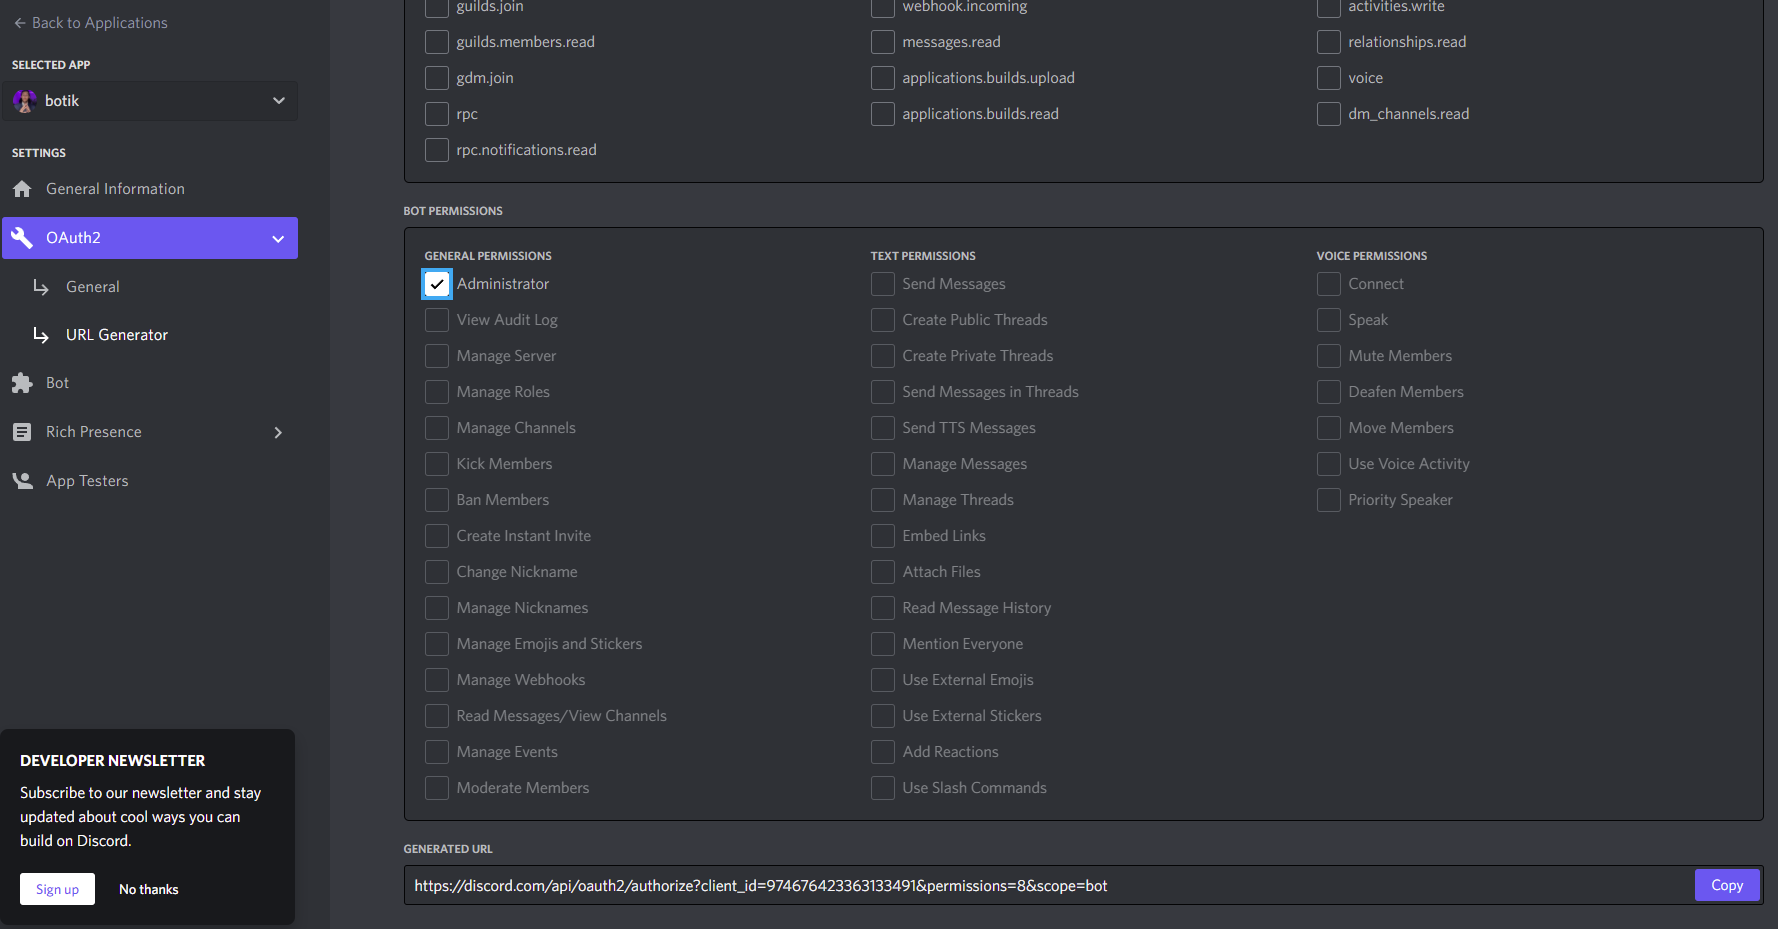
\includegraphics[width = 450px]{pictures/oauth2.png}}


\newpage
\subsection{Активация бота и его тестирование}
\noindent
Для начала работы с кодом нам нужно установить среду разработки. \\ 
Среда разработки выбирается по удобству использования и практичности, я выбрал Visual Studio Code \\

\noindent
Для создания бота используем среду выполнения node.js \\

\noindent
\begin{center}
\textbf{Подготовка к написанию кода}\\
\end{center}
\begin{itemize}
    \item Первым делом создаём папку, после чего открываем её в VS Code
    \item Теперь создаём файл с неким «описанием» нашего бота, сделаем это через терминал.
    Вписываем данную строку в терминал: \textbf{npm init} \\
    После каждой появившейся строки нажимаем Enter или вписываем свои значения.
    Значения в этом файле можно будет изменить в любой момент.
    \item Устанавливаем нужные пакеты и модули, чтобы в дальнейшем наш бот корректно работал. \\
    Поочерёдно вводим следующие команды: \textbf{ \\npm install \\ npm install discord.js axios dotenv}
    \item Итого, в нашей папке появляется 3 объекта: nodeModules, package.json, package-lock.json
\end{itemize}

\newpage
\begin{center}
\textbf{Написание кода}\\
\end{center}

Для того, чтобы наш бот появился в сети и мог реагировать на команды, нам нужно написать для него код.\\

Код будем писать используя два файла, чтобы легко ориентироваться, один для запуска бота, другой для создания команд (также есть и другие файлы, но к ним редко приходиться обращаться) \\

\begin{itemize}
    \item Для начала создадим файл config.json, который будет содержать токен нашего бота и префикс (символ который нужно будет приписать к команде, чтобы бот отреагировал на наше сообщение)
    \item Далее создаём файл для запуска бота, назовём его bot.js
    \item Напишем для него код, а именно подключаем его к библиотекам, работаем с префиксом и токеном, создаём функцию которая нам поможет понять работает бот или нет, а также функцию реагирования на наши сообщения
    \item Теперь создаём файл comms.js, в нём будут сами команды.
    \item Также подключаем к биоблетекам и связываем с bot.js, выстаскиваем префикс
    \item Пишем первую команду, для того чтобы протестировать что бот работает и формируем список команд, для вызова команды в чате
\end{itemize}


\centerline{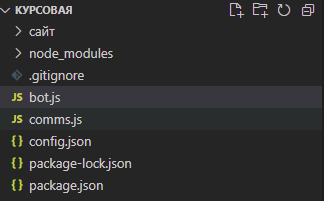
\includegraphics[width = 350px]{pictures/papki.png}} \\
\vspace{10mm}
\centerline{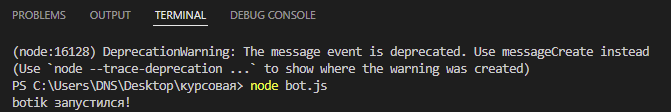
\includegraphics[width = 500px,height = 130px]{pictures/zap.png}} \\
\vfill
\newpage
\centerline{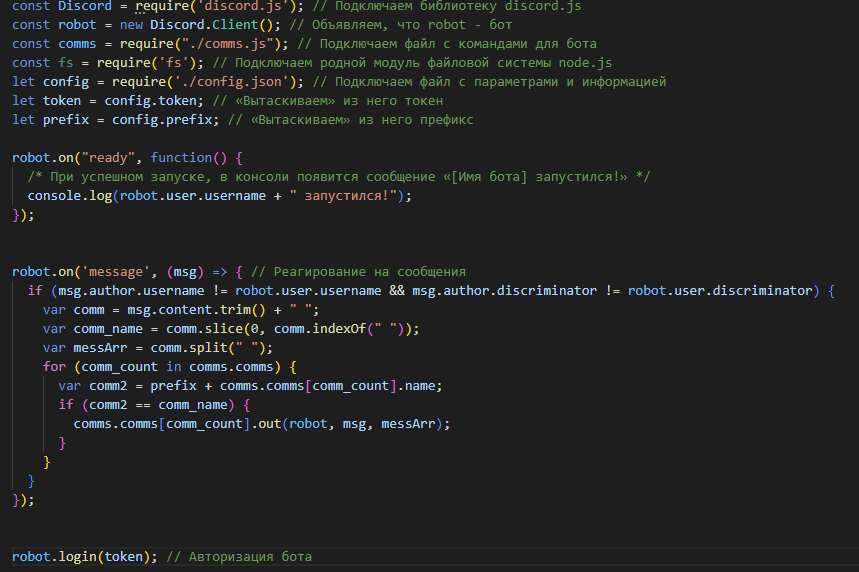
\includegraphics[width = 450px,height = 300px]{pictures/kod.png}} \\
\vspace{10mm}
\centerline{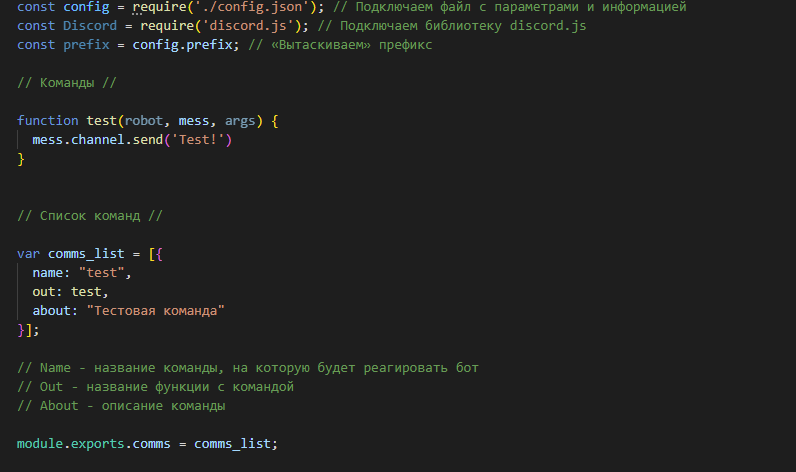
\includegraphics[width = 450px,height = 300px]{pictures/kod2.png}}
\vfill


\newpage
\subsection{Добавление большего функционала (добавляем команды)}
Бот запущен и вы можете им пользоваться, а значит можно приступить к добавлению новых команд

\begin{itemize}
    \item Начнём с своеобразного Флешфорварда, создаём команду help которая будет выводить все наши команды, это необходимо для того чтобы новые пользователи могли ознакомиться с функционалом бота
    \centerline{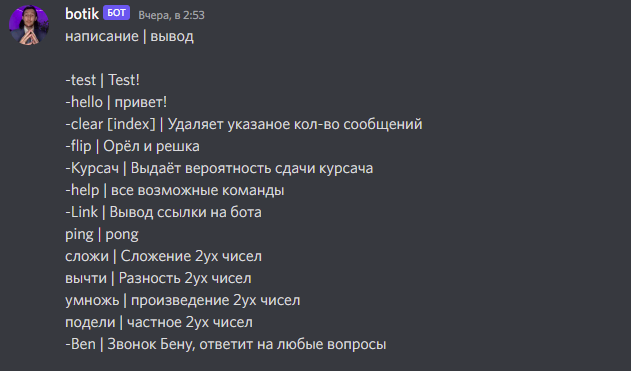
\includegraphics[width = 450px,height = 300px]{pictures/help.png}}
    \item Первая команда которую мы создадим (после теста конечно), будет своеобразным Hello World! \\
    \centerline{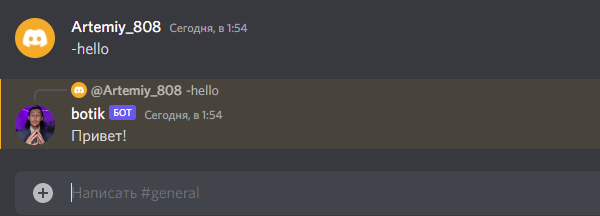
\includegraphics[width = 350px]{pictures/hello.png}}
\newpage
    \item Следующая команда будет удалять конкретное кол-во сообщений указанное нами \\
    \centerline{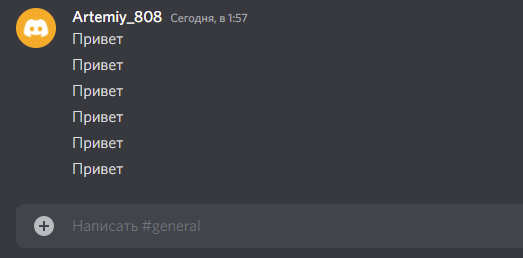
\includegraphics[width = 200px]{pictures/do.png}\\ 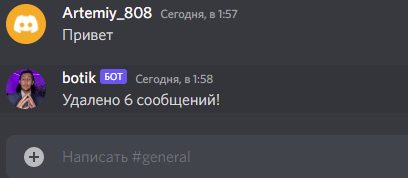
\includegraphics[width = 230px]{pictures/posle.png}}
    \item Для того чтобы разрешать споры между нашими дорогими пользователями сделана команда flip или же орёл и решка, при вызове команды выпадает одно из трёх состояний: Орёл, Ребро, Решка \\
    \centerline{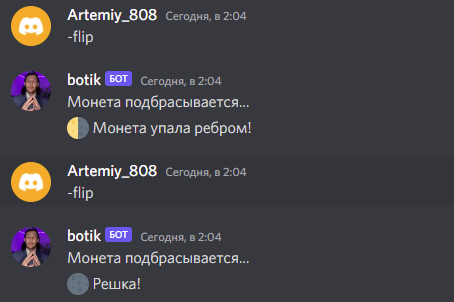
\includegraphics[width = 300px]{pictures/flip.png}}
    \item Команда для того чтобы получить ссылку на бота, который можно поделиться со своим другом, мамой, папой, бабушкой имя её link \\
    \centerline{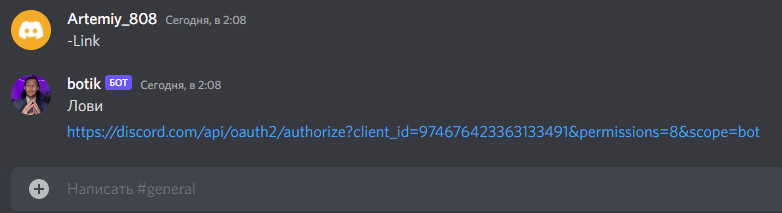
\includegraphics[width = 450px]{pictures/Link.png}}
\newpage
    \item Далее чтобы скоротать ожидание сдачи курсовой работы была создана команда Курсач, которая выдаёт вероятность сдачи курсовой
    \centerline{
\includegraphics[width = 450px]{pictures/kurs.png}}
    Вау, мне повезло и моя вероятность сдачи курсовой 100 процентов!!! (после сотого вызова команды)
    \item Сидите дома, а хочется позаниматься спортом, тогда для вас команда ping(по сути что и test, но для неё не нужен префикс), на неё бот ответит pong и так можно своеобразно играть в ping-pong
    \centerline{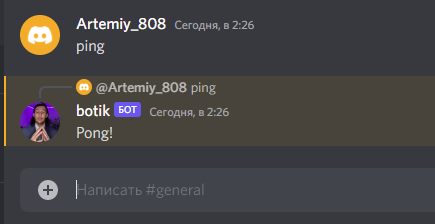
\includegraphics[width = 350px]{pictures/ping.png}} \\
\newpage
    \item Если вдруг у вас нету калькулятора под рукой, а вы забыли простейшие правила вычитания, сложения, умножения и деления, то можно воспользоваться следующими комаднам: сложи, вычти, умножь и подели \\
    \centerline{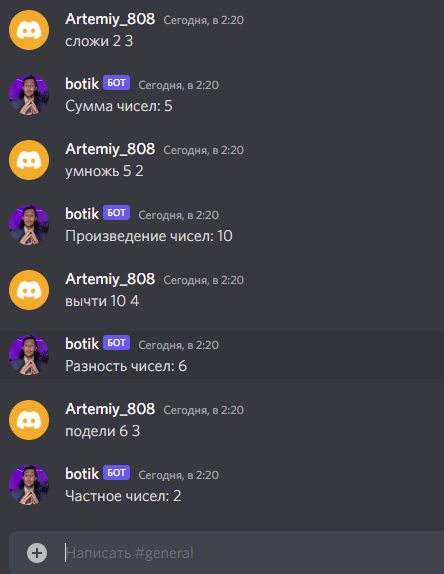
\includegraphics[width = 400px]{pictures/math.png}} \\
    Ещё важная особенность этих команд что для них не нужно использовать префикс
\newpage
    \item Ну и последняя команда -Ben, в сети разверусилась старая мобильная игра my talking ben, ему можно позвонить и он будет давать вам 4 ответа да, нет, отвращение и смех, я решил добавить своеобразную версию "Ben`a" в функционал своего бота, картинки он не имеет, но на сообщения отвечает \\
    \centerline{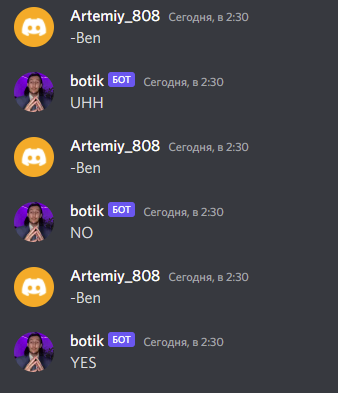
\includegraphics[width = 350px]{pictures/Ben.png}}
\end{itemize}

\newpage
\section{Создание сайта}
Для того чтобы человек не имеющий ссылки мог скачать бота, создадим сайт в котором будет кнопка с url-ссылкой

\begin{center}
\textbf{Сайт имеет следующий вид:}
\end{center}
\centerline{\includegraphics[width = 200px]{pictures/Site.png}\\ 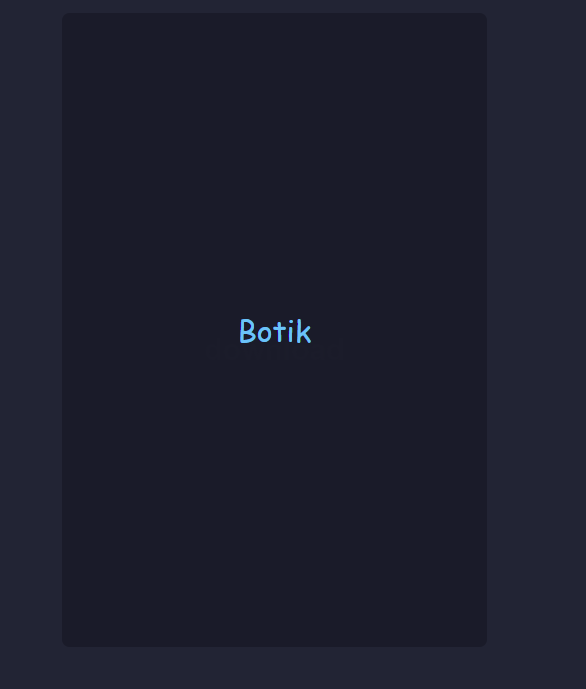
\includegraphics[width = 200px]{pictures/site2.png}}
Представляет собой карту с красивой анимацией, при навождении на неё освещение пропадает, как бы отдавая свою энергию тексту, из-за чего он появляется, а по нажатию нам предлагают загрузить бота на наш сервер
\centerline{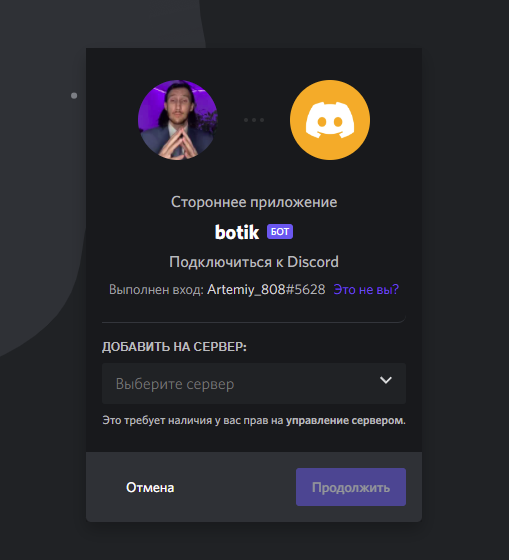
\includegraphics[width = 230px]{pictures/linklink.png}}

\newpage
\section{Вывод}
\Large
В своей курсовой работе была рассмотрена работа с Discord для разработчиков, а именно создание discord bot`а, от добавления его на собственный сервер, до активирования с небольшим количеством команд, которым могут пользоваться другие пользователи. В ходе работы был получен опыт работы с Node.js, API, JavaScript, Discord for Developer, JSON, а также закрепление полученных навыков работы с CSS, HTML, GitHub, Latex, Beamer. \\

Болшинство поставленных задач было выполнено, за исключение более глубокой работы с API, например подключение к другому сайту с целью вывода картинки по команде в текстовый канал Discord\\ \\


\newpage
\large
\begin{thebibliography}{100}

\section{Список литературы}
\bibitem{Discord.js} Основная документация discord.js — URL: https://discord.js.org/#/
\bibitem{Discord.js2} Документация discord.js №2 — URL: https://discordjs-fork.readthedocs.io/en/latest/index.html
\bibitem{Discord.js3} Руководство discord.js — URL: https://discordjs.guide/#before-you-begin
\bibitem{Discord.js4} Руководство discord.js №2 — URL: https://anidiots.guide/
\bibitem{Discord.js5} Discord developers — URL: https://discord.com/developers
\bibitem{Node.js} Node.js — URL: https://nodejs.org/en/
\bibitem{VScode} Visual Studio Code — URL: https://code.visualstudio.com/
\end{thebibliography}

%%%                          %%%
%%%%%%%%%%%%%%%%%%%%%%%%%%%%%%%%

\end{document}
